\documentclass[12pt]{extreport}
\usepackage[T2A]{fontenc}
\usepackage[utf8]{inputenc}        % Кодировка входного документа;
                                    % при необходимости, вместо cp1251
                                    % можно указать cp866 (Alt-кодировка
                                    % DOS) или koi8-r.

\usepackage[english,russian]{babel} % Включение русификации, русских и
                                    % английских стилей и переносов
%%\usepackage{a4}
%%\usepackage{moreverb}
\usepackage{amsmath,amsfonts,amsthm,amssymb,amsbsy,amstext,amscd,amsxtra,multicol}
\usepackage{indentfirst}
\usepackage{verbatim}
\usepackage{tikz} %Рисование автоматов
\usetikzlibrary{automata,positioning}
\usepackage{multicol} %Несколько колонок
\usepackage{graphicx}
\usepackage[colorlinks,urlcolor=blue]{hyperref}
\usepackage[stable]{footmisc}

\usepackage[linesnumbered]{algorithm2e}   

%% \voffset-5mm
%% \def\baselinestretch{1.44}
\renewcommand{\theequation}{\arabic{equation}}
\def\hm#1{#1\nobreak\discretionary{}{\hbox{$#1$}}{}}
\newtheorem{Lemma}{Лемма}
\theoremstyle{definiton}
\newtheorem{Remark}{Замечание}
%%\newtheorem{Def}{Определение}
\newtheorem{Claim}{Утверждение}
\newtheorem{Cor}{Следствие}
\newtheorem{Theorem}{Теорема}
\theoremstyle{definition}
\newtheorem{Example}{Пример}
\newtheorem*{known}{Теорема}
\def\proofname{Доказательство}
\theoremstyle{definition}
\newtheorem{Def}{Определение}

%% \newenvironment{Example} % имя окружения
%% {\par\noindent{\bf Пример.}} % команды для \begin
%% {\hfill$\scriptstyle\qed$} % команды для \end






%\date{22 июня 2011 г.}
\let\leq\leqslant
\let\geq\geqslant
\def\MT{\mathrm{MT}}
%Обозначения ``ажуром''
\def\BB{\mathbb B}
\def\CC{\mathbb C}
\def\RR{\mathbb R}
\def\SS{\mathbb S}
\def\ZZ{\mathbb Z}
\def\NN{\mathbb N}
\def\FF{\mathbb F}
%греческие буквы
\let\epsilon\varepsilon
\let\es\varnothing
\let\eps\varepsilon
\let\al\alpha
\let\sg\sigma
\let\ga\gamma
\let\ph\varphi
\let\om\omega
\let\ld\lambda
\let\Ld\Lambda
\let\vk\varkappa
\let\Om\Omega
\def\abstractname{}

\def\R{{\cal R}}
\def\A{{\cal A}}
\def\B{{\cal B}}
\def\C{{\cal C}}
\def\D{{\cal D}}

%классы сложности
\def\REG{{\mathsf{REG}}}
\def\CFL{{\mathsf{CFL}}}


%%%%%%%%%%%%%%%%%%%%%%%%%%%%%%% Problems macros  %%%%%%%%%%%%%%%%%%%%%%%%%%%%%%%


%%%%%%%%%%%%%%%%%%%%%%%% Enumerations %%%%%%%%%%%%%%%%%%%%%%%%

\newcommand{\Rnum}[1]{\expandafter{\romannumeral #1\relax}}
\newcommand{\RNum}[1]{\uppercase\expandafter{\romannumeral #1\relax}}

%%%%%%%%%%%%%%%%%%%%% EOF Enumerations %%%%%%%%%%%%%%%%%%%%%

\usepackage{xparse}
\usepackage{ifthen}
\usepackage{bm} %%% bf in math mode
\usepackage{color}
%\usepackage[usenames,dvipsnames]{xcolor}

\definecolor{Gray555}{HTML}{555555}
\definecolor{Gray444}{HTML}{444444}
\definecolor{Gray333}{HTML}{333333}


\newcounter{problem}
\newcounter{uproblem}
\newcounter{subproblem}
\newcounter{prvar}

\def\beforPRskip{
	\bigskip
	%\vspace*{2ex}
}

\def\PRSUBskip{
	\medskip
}


\def\pr{\beforPRskip\noindent\stepcounter{problem}{\bf \theproblem .\;}\setcounter{subproblem}{0}}
\def\pru{\beforPRskip\noindent\stepcounter{problem}{\bf $\mathbf{\theproblem}^\circ$\!\!.\;}\setcounter{subproblem}{0}}
\def\prstar{\beforPRskip\noindent\stepcounter{problem}{\bf $\mathbf{\theproblem}^*$\negthickspace.}\setcounter{subproblem}{0}\;}
\def\prpfrom[#1]{\beforPRskip\noindent\stepcounter{problem}{\bf Задача \theproblem~(№#1 из задания).  }\setcounter{subproblem}{0} }
\def\prp{\beforPRskip\noindent\stepcounter{problem}{\bf Задача \theproblem .  }\setcounter{subproblem}{0} }

\def\prpvar{\beforPRskip\noindent\stepcounter{problem}\setcounter{prvar}{1}{\bf Задача \theproblem \;$\langle${\rm\Rnum{\theprvar}}$\rangle$.}\setcounter{subproblem}{0}\;}
\def\prpv{\beforPRskip\noindent\stepcounter{prvar}{\bf Задача \theproblem \,$\bm\langle$\bracketspace{{\rm\Rnum{\theprvar}}}$\bm\rangle$.  }\setcounter{subproblem}{0} }
\def\prv{\beforPRskip\noindent\stepcounter{prvar}{\bf \theproblem\,$\bm\langle$\bracketspace{{\rm\Rnum{\theprvar}}}$\bm\rangle$}.\setcounter{subproblem}{0} }

\def\prpstar{\beforPRskip\noindent\stepcounter{problem}{\bf Задача $\bf\theproblem^*$\negthickspace.  }\setcounter{subproblem}{0} }
\def\prdag{\beforPRskip\noindent\stepcounter{problem}{\bf Задача $\theproblem^{^\dagger}$\negthickspace\,.  }\setcounter{subproblem}{0} }
\def\upr{\beforPRskip\noindent\stepcounter{uproblem}{\bf Упражнение \theuproblem.}\setcounter{subproblem}{0}\;}
%\def\prp{\vspace{5pt}\stepcounter{problem}{\bf Задача \theproblem .  } }
%\def\prs{\vspace{5pt}\stepcounter{problem}{\bf \theproblem .*   }
\def\prsub{\PRSUBskip\noindent\stepcounter{subproblem}{\sf \thesubproblem.}\;}
\def\prsubr{\PRSUBskip\noindent\stepcounter{subproblem}{\bf \asbuk{subproblem})}\;}
\def\prsubstar{\PRSUBskip\noindent\stepcounter{subproblem}{\rm $\thesubproblem^*$\negthickspace.}\;}
\def\prsubrstar{\PRSUBskip\noindent\stepcounter{subproblem}{$\text{\bf \asbuk{subproblem}}^*\mathbf{)}$}\;}

\newcommand{\bracketspace}[1]{\phantom{(}\!\!{#1}\!\!\phantom{)}}

\DeclareDocumentCommand{\Prpvar}{ O{null} O{} }{
	\beforPRskip\noindent\stepcounter{problem}\setcounter{prvar}{1}{\bf Задача \theproblem
% 	\ifthenelse{\equal{#1}{null}}{  }{ {\sf $\bm\langle$\bracketspace{#1}$\bm\rangle$}}
%	~\!\!(\bracketspace{{\rm\Rnum{\theprvar}}}).  }\setcounter{subproblem}{0}
%	\;(\bracketspace{{\rm\Rnum{\theprvar}}})}\setcounter{subproblem}{0}
%
	\,{\sf $\bm\langle$\bracketspace{{\rm\Rnum{\theprvar}}}$\bm\rangle$}
	~\!\!\! \ifthenelse{\equal{#1}{null}}{\!}{{\sf(\bracketspace{#1})}}}.

}
%\DeclareDocumentCommand{\Prpvar}{ O{level} O{meta} m }{\prpvar}


\DeclareDocumentCommand{\Prp}{ O{null} O{null} }{\setcounter{subproblem}{0}
	\beforPRskip\noindent\stepcounter{problem}\setcounter{prvar}{0}{\bf Задача \theproblem
	~\!\!\! \ifthenelse{\equal{#1}{null}}{\!}{{\sf(\bracketspace{#1})}}
	 \ifthenelse{\equal{#2}{null}}{\!\!}{{\sf [\color{Gray444}\,\bracketspace{{\fontfamily{afd}\selectfont#2}}\,]}}}.}

\DeclareDocumentCommand{\Pr}{ O{null} O{null} }{\setcounter{subproblem}{0}
	\beforPRskip\noindent\stepcounter{problem}\setcounter{prvar}{0}{\bf\theproblem
	~\!\! \ifthenelse{\equal{#1}{null}}{\!\!}{{\sf(\bracketspace{#1})}}
	 \ifthenelse{\equal{#2}{null}}{\!\!}{{\sf [\color{Gray444}\,\bracketspace{{\fontfamily{afd}\selectfont#2}}\,]}}}.}
	
	\DeclareDocumentCommand{\Prstar}{ O{null} O{null} }{\setcounter{subproblem}{0}
			\medskip\noindent\stepcounter{problem}\setcounter{prvar}{0}{\bf$\mathbf{\theproblem^*}$
			~\!\!\! \ifthenelse{\equal{#1}{null}}{\!}{{\sf(\bracketspace{#1})}}
			 \ifthenelse{\equal{#2}{null}}{\!\!}{{\sf [\color{Gray444}\,\bracketspace{{\fontfamily{afd}\selectfont#2}}\,]}}}.}
	

%\DeclareDocumentCommand{\Prp}{ O{level} O{meta} }

\DeclareDocumentCommand{\Prps}{ O{null} O{null} }{\setcounter{subproblem}{0}
	\beforPRskip\noindent\stepcounter{problem}\setcounter{prvar}{0}{\bf Задача $\bm\theproblem^* $
	~\!\!\! \ifthenelse{\equal{#1}{null}}{\!}{{\sf(\bracketspace{#1})}}
	 \ifthenelse{\equal{#2}{null}}{\!\!}{{\sf [\color{Gray444}\,\bracketspace{{\fontfamily{afd}\selectfont#2}}\,]}}}.
}

\DeclareDocumentCommand{\Prpd}{ O{null} O{null} }{\setcounter{subproblem}{0}
	\beforPRskip\noindent\stepcounter{problem}\setcounter{prvar}{0}{\bf Задача $\bm\theproblem^\dagger$
	~\!\!\! \ifthenelse{\equal{#1}{null}}{\!}{{\sf(\bracketspace{#1})}}
	 \ifthenelse{\equal{#2}{null}}{\!\!}{{\sf [\color{Gray444}\,\bracketspace{{\fontfamily{afd}\selectfont#2}}\,]}}}.
}


\def\prend{
	\bigskip
%	\bigskip
}




%%%%%%%%%%%%%%%%%%%%%%%%%%%%%%% EOF Problems macros  %%%%%%%%%%%%%%%%%%%%%%%%%%%%%%%



%\usepackage{erewhon}
%\usepackage{heuristica}
%\usepackage{gentium}

\usepackage[portrait, top=3cm, bottom=1.5cm, left=3cm, right=2cm]{geometry}

\usepackage{fancyhdr}
\pagestyle{fancy}
% \renewcommand{\headrulewidth}{0pt}
\lhead{\fontfamily{fca}\selectfont {\color{myblue}\bf{Шарипов Саит}} }
\rhead{\fontfamily{fca}\selectfont {Задачи разрешимости логических формул и приложения\ \ \ \  ДЗ№2} }
% \rhead{\fontfamily{fca}\selectfont ДЗ№1}
%\lhead{ \bf  {ТРЯП. } Семинар 1 }
%\chead{\fontfamily{fca}\selectfont {Вариант 1}}
%\rhead{\small 01.09.2016}
\cfoot{}

\usepackage{titlesec}
\titleformat{\section}[block]{\Large\bfseries\filcenter {\setcounter{problem}{0}}  }{}{1em}{}


%%%%%%%%%%%%%%%%%%%%%%%%%%%%%%%%%%%%%%%%%%%%%%%%%%%% Обозначения и операции %%%%%%%%%%%%%%%%%%%%%%%%%%%%%%%%%%%%%%%%%%%%%%%%%%%% 
                                                                    
\newcommand{\divisible}{\mathop{\raisebox{-2pt}{\vdots}}}           
\let\Om\Omega


%%%%%%%%%%%%%%%%%%%%%%%%%%%%%%%%%%%%%%%% Shen Macroses %%%%%%%%%%%%%%%%%%%%%%%%%%%%%%%%%%%%%%%%
\newcommand{\w}[1]{{\hbox{\texttt{#1}}}}
\usepackage{wrapfig}
\def\bin{\mathrm{bin}}

% МОЙ КОД НАЧАЛО
\definecolor{myblue}{RGB}{0, 0, 102}
\definecolor{myyellow}{RGB}{252, 245, 174}

\newcommand{\solution}[2][\color{myblue}Решение]{
\medskip
	\noindent{\bfseries #1 }{{\color{myblue}\bfseries #2:}}
%\medskip	
}

\newenvironment{blockquote}{%
  \par%
  \medskip
  \leftskip=1em%
  \noindent}{%
  \par\medskip}
  
\usepackage{listings}
\usepackage{xcolor}
\lstset { %
    language=C++,
    belowcaptionskip=1\baselineskip,
    breaklines=true,
    frame=L,
    xleftmargin=\parindent,
    language=C,
    showstringspaces=false,
    basicstyle=\footnotesize\ttfamily,
    keywordstyle=\bfseries\color{purple!40!black},
    commentstyle=\itshape\color{green!40!black},
    identifierstyle=\color{blue},
    stringstyle=\color{orange},
    backgroundcolor=\color{black!5}, % set backgroundcolor
    basewidth=0.5em,
    numbers=left,
}
\usepackage{subcaption}
\usepackage{float}
% МОЙ КОД КОНЕЦ



\begin{document}	
\SetKwFunction{BuildMaxHeap}{Build\_Max\_Heap} 
\SetKwFunction{TreeSuccessor}{Tree\_Successor} 
\SetKwFunction{ExtMax}{Extract\_Max} 
\SetKwFunction{MaxHeapify}{Max\_Heapify}

\SetKwInOut{Input}{Вход}\SetKwInOut{Output}{Выход}
\SetKwProg{Fn}{Function}{ :}{end}
\SetKwFunction{F}{F}
\SetKwFunction{KWsize}{size}
\SetKwFunction{HeapSize}{heap\_size}
\SetKwFunction{KwPrint}{print} 
\SetKwFunction{swap}{swap}
			
% Задача №1			
\Pr[10 баллов] Напишите генератор формулы colorA($n$) в формате DIMACS для задачи о том, что существует $2$-раскраска положительных чисел от $1$ до $n$ такая, что для любого целочисленного решения $a + b = c$ т.ч. $1 \leq a < b < c \leq n$ выполняется, что $a$, $b$ и $c$ не имеют одинаковый цвет.\\
\textbf{\textit{Подсказка:}} для каждого целого числа используйте булеву переменную $x_i$. $x_i$ равно $true$ означает, что $i$ раскрашено в первый цвет, и равно $false$, если $i$ раскрашен во второй цвет.
			
\solution{1}
\begin{blockquote}
{\color{myblue}
\noindent Для каждого числа $i$ ($1 \leq i \leq n$) введем переменную $x_i$ следующим образом:
\begin{equation*}
x_i = 
 \begin{cases}
   true, &\text{если число $i$ раскрашено в первый цвет}\\
   false, &\text{если число $i$ раскрашено во второй цвет}
 \end{cases}
\end{equation*}
Тогда, будем перебирать числа $a$, $b$ и $c$ ($1 \leq a < b < c \leq n$), и в случае, если выполняется, что $a + b = c$ требовать, чтобы выполнялось условие:
$$\overline{(x_a \wedge x_b \wedge x_c) \vee (\overline{x_a} \wedge \overline{x_b} \wedge \overline{x_c})}$$
Поскольку:\\
$x_a \wedge x_b \wedge x_c$ равно $true$ $\Leftrightarrow$ если $a$, $b$ и $c$ все имеют первый цвет;\\ $\overline{x_a} \wedge \overline{x_b} \wedge \overline{x_c}$ равно $true$ $\Leftrightarrow$ если $a$, $b$ и $c$ все имеют второй цвет;\\
$(x_a \wedge x_b \wedge x_c) \vee (\overline{x_a} \wedge \overline{x_b} \wedge \overline{x_c})$ равно $true$ $\Leftrightarrow$ если $a$, $b$ и $c$ имеют одинаковый цвет (первый или второй);\\
$\overline{(x_a \wedge x_b \wedge x_c) \vee (\overline{x_a} \wedge \overline{x_b} \wedge \overline{x_c})}$ равно $true$ $\Leftrightarrow$ если $a$, $b$ и $c$ не имеют одинаковый цвет;\\
\\
Теперь следует преобразовать это к КНФ:
$$\overline{(x_a \wedge x_b \wedge x_c) \vee (\overline{x_a} \wedge \overline{x_b} \wedge \overline{x_c})} = (\overline{x_a} \vee \overline{x_b} \vee \overline{x_c}) \wedge (x_a \vee x_b \vee x_c)$$
Осталось вспомнить правила записи КНФ в DIMACS формате:
\begin{itemize}
    \item \textit{Комментарий}: \textbf{c <comment>}
    \item \textit{Заголовок}: \textbf{p cnf <n> <m>}, где $n$ - количество переменных, $m$ - количество дизъюнктов.
    \item \textit{Описание дизъюнкта}: номера переменных через пробел, со знаком $-$, если переменная с отрицанием. В конце дизъюнкта всегда 0.
    \item \textit{Пример КНФ}: $(x_1 \vee x_2 \vee \overline{x_3}) \wedge (\overline{x_1} \vee \overline{x_2} \vee x_3) \wedge (x_2 \vee x_3 \vee \overline{x_4})$.
    \item \textit{DIMACS формат для примера:}\\
    c example\\
    p cnf 4 3\\
    1 2 -3 0\\
    -1 -2 3 0\\
    2 3 -4 0\\
\end{itemize}
Генератор формулы colorA($n$) находится в программе {\fcolorbox{red}{myyellow}{01\_colorA.py}}.
}
\end{blockquote}

% Задача №2
\Pr[10 баллов] Напишите генератор формулы colorB($n$) в DIMACS формат для задачи о том, что существует $2$-раскраска положительных чисел от $1$ до $n$ такая, что для любого целочисленного решения $a^2+b^2 =c^2$ $(1 \leq a < b < c \leq n)$ выполняется, что $a$, $b$ и $c$ не имеют одинаковый цвет.

\solution{2}
\begin{blockquote}
{\color{myblue}
\noindent Данная задача имеет ту же идею решения, что и задача №$1$.
Отличие заключается в том, как будет организован перебор троек чисел $a$, $b$ и $c$. Будем перебирать числа $a$, $b$ и $c$ ($1 \leq a < b < c \leq n$), и в случае, если выполняется, что $a^2 + b^2 = c^2$ требовать, чтобы выполнялось условие:
$$(\overline{x_a} \vee \overline{x_b} \vee \overline{x_c}) \wedge (x_a \vee x_b \vee x_c)$$
Генератор формулы colorB($n$) находится в программе {\fcolorbox{red}{myyellow}{02\_colorB.py}}.
}
\end{blockquote}

% Задача №3
\Pr[10 баллов] Используйте указанный выше генератор, чтобы построить формулу colorA($7$). Рассмотрим начальные шаги CDCL, в которых $x_1 = 1, x_3 = 1$. Распространение единиц приводит к конфликту. Нарисуйте граф импликации и вычислите первую уникальную точку импликации этого графа.

\solution{3}
\begin{blockquote}
{\color{myblue}
\noindent Результат генератора из задачи №$1$ для colorA($7$):\\
\begin{lstlisting}
c colorA(7)
p cnf 7 18
-1 -2 -3 0
1 2 3 0
-1 -3 -4 0
1 3 4 0
-1 -4 -5 0
1 4 5 0
-1 -5 -6 0
1 5 6 0
-1 -6 -7 0
1 6 7 0
-2 -3 -5 0
2 3 5 0
-2 -4 -6 0
2 4 6 0
-2 -5 -7 0
2 5 7 0
-3 -4 -7 0
3 4 7 0
\end{lstlisting}
Таким образом, мы имеем следующую систему дизъюнктов:\\
$c_1 = (\neg x_1 \vee \neg x_2 \vee \neg x_3)$\\ % 3 строчка
$c_2 = (x_1 \vee x_2 \vee x_3)$\\ % 4 строчка
$c_3 = (\neg x_1 \vee \neg x_3 \vee \neg x_4)$\\ % 5 строчка
$c_4 = (x_1 \vee x_3 \vee x_4)$\\ % 6 строчка
$c_5 = (\neg x_1 \vee \neg x_4 \vee \neg x_5)$\\ % 7 строчка
$c_6 = (x_1 \vee x_4 \vee x_5)$\\ % 8 строчка
$c_7 = (\neg x_1 \vee \neg x_5 \vee \neg x_6)$\\ % 9 строчка
$c_8 = (x_1 \vee x_5 \vee x_6)$\\ % 10 строчка
$c_9 = (\neg x_1 \vee \neg x_6 \vee \neg x_7)$\\ % 11 строчка
$c_{10} = (x_1 \vee x_6 \vee x_7)$\\ % 12 строчка
$c_{11} = (\neg x_2 \vee \neg x_3 \vee \neg x_5)$\\ % 13 строчка
$c_{12} = (x_2 \vee x_3 \vee x_5)$\\ % 14 строчка
$c_{13} = (\neg x_2 \vee \neg x_4 \vee \neg x_6)$\\ % 15 строчка
$c_{14} = (x_2 \vee x_4 \vee x_6)$\\ % 16 строчка
$c_{15} = (\neg x_2 \vee \neg x_5 \vee \neg x_7)$\\ % 17 строчка
$c_{16} = (x_2 \vee x_5 \vee x_7)$\\ % 18 строчка
$c_{17} = (\neg x_3 \vee \neg x_4 \vee \neg x_7)$\\ % 19 строчка
$c_{18} = (x_3 \vee x_4 \vee x_7)$\\ % 20 строчка
\\
\textbf{\textit{Conflict-driven clause learning (CDCL)}}:
\begin{itemize}
    \item Изначально, пока не сделали ни одно предположение находимся на нулевом уровне.
    \item Каждое предположение о значении переменной порождает новый уровень.
    \item Будем писать $x_i @ dl$, если на уровне принятия решений $dl$ мы присвоили переменной $x_i$ значение истина и $\neg{x_i}  @ dl$ - если присвоили ложь.
    \item Вершины графа - переменные, определенные частичной оценкой.
    \item Из вершины $v_i$ идет ребро в вершину $v_j$ , если переменная $v_j$ оценена в результате $BCP()$ и $v_i$ входит в дизъюнкт-предпосылку $c$. Это ребро помечается меткой $c$.
    \item Если есть конфликт, то ему соответствует вершина \textbf{К}. Пусть $c$ - конфликтный дизъюнкт. Тогда к вершине \textbf{К} идут ребра от переменных, входящих в $c$ и они помечаются меткой $c$.
    \item При возникновении конфликта откатываемся к предпоследнему уровню, эксперименты показывают, что так быстрее.
    \item \textit{Уникальная точка импликации} -- любая вершина графа импликации, которая не является вершиной «конфликт» и которая находится на каждом пути, ведущему от конкретной корневой вершины к конкретной вершине «конфликт».
    \item \textit{Первая УТИ} -- ближайшая к конфликтной вершине уникальная точка импликации.
\end{itemize}
На рисунке~\ref{ris:cdcl} представлен граф импликации.
\begin{figure}[H]
    \centering
    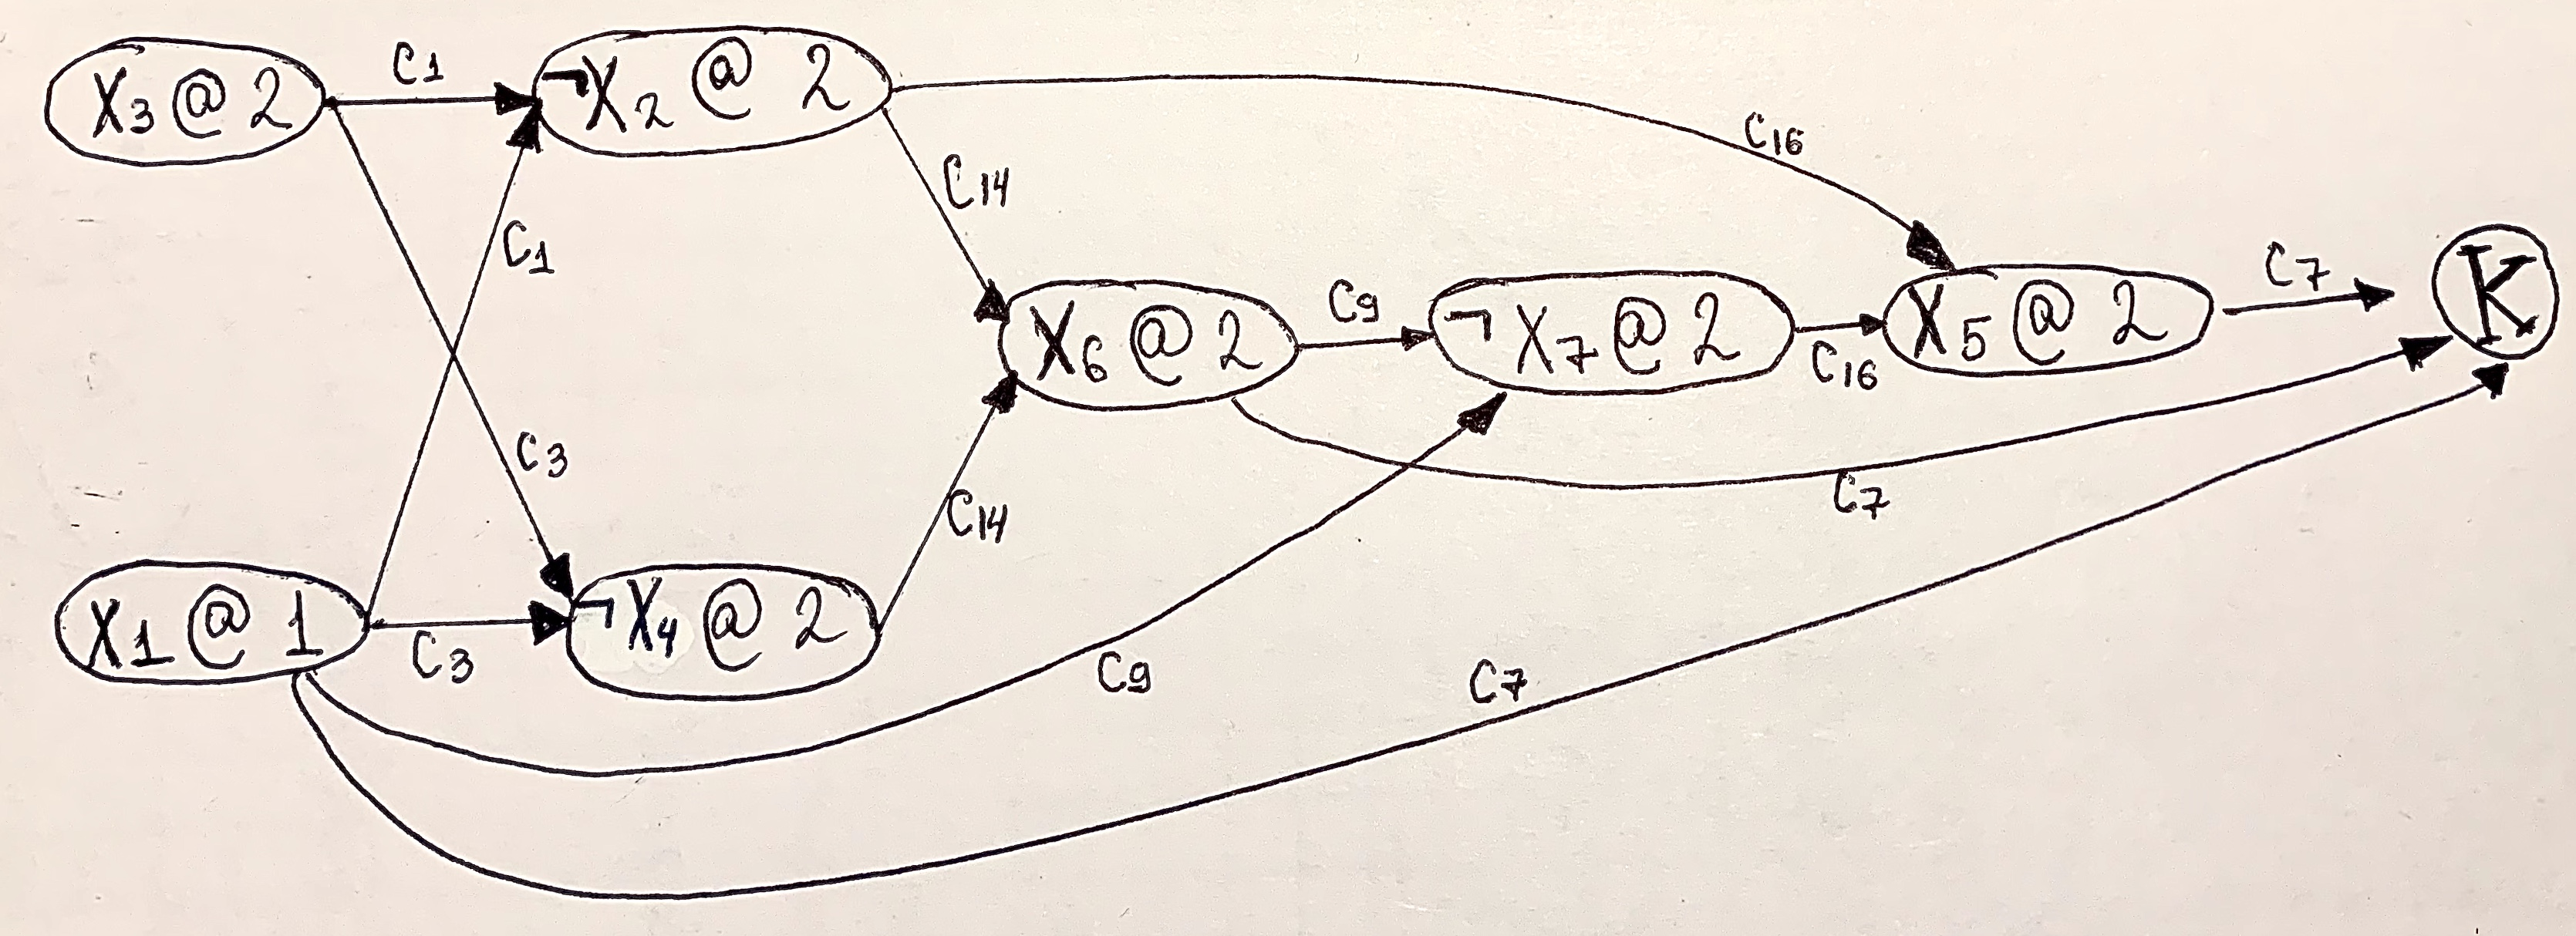
\includegraphics[width=16.5cm]{images/cdcl.JPG}
    \caption{Граф импликации для задачи $3$.}
    \label{ris:cdcl}
\end{figure}

Видим, что:
\begin{itemize}
    \item Первая УТИ для корневой вершины \textbf{$x_1 @ 1$} -- вершина \textbf{$x_1 @ 1$}.
    \item Первая УТИ для корневой вершины \textbf{$x_3 @ 2$} -- вершина \textbf{$x_3 @ 2$}.
\end{itemize}



}
\end{blockquote}

% Задача №4
\Pr[10 баллов] Напишите общий генератор DIMACS для головоломок $n$-судоку, т.е. для пустого поля.\\
\textbf{\textit{Пояснение:}} $n$-судоку -- это значит, что дано поле $n^2 \times n^2$, которое разбито на квадраты размера $n \times n$. В каждой строчке, столбце, квадрате  может быть не более одного числа от $1$ до $n^2$. Поля $2$-судоку и $3$-судоку представлены на первом и втором рисунках ниже:
\begin{minipage}{.49\textwidth}
  \centering
  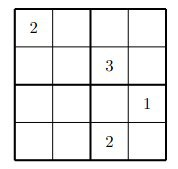
\includegraphics[width=4.5cm]{images/sudoku3.jpg}{\\$2$-судоку.}
%   \caption{$2$-судоку.}
\end{minipage}
\begin{minipage}{.49\textwidth}
  \centering
  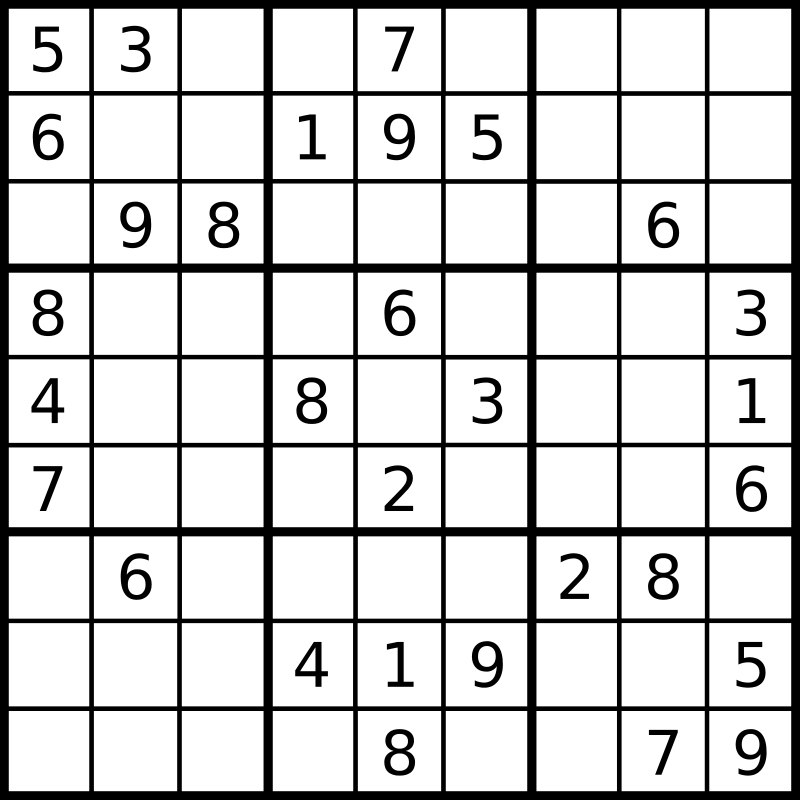
\includegraphics[width=4.0cm]{images/sudocu2.jpg}{\\$3$-судоку.}
%   \caption{$3$-судоку.}
\end{minipage}

\solution{4}
\begin{blockquote}
{\color{myblue}
\noindent Будем кодировать $n$-судоку следующим образом ($1 \leq i, j, k \leq n^2$):
\begin{equation*}
x_{ij}^k = 
 \begin{cases}
   true, &\text{если в $n$-судоку в клетке $i$, $j$ стоит число $k$}\\
   false, &\text{если в $n$-судоку в клетке $i$, $j$ стоит число не $k$}
 \end{cases}
\end{equation*}
Таким образом для каждой клетки $n$-судоку будет $n^2$ переменных, а всего будет\\ $n^2 \cdot n^2 \cdot n^2 = n^6$ переменных.\\
\\
Для начала зафиксируем правило расстановки чисел в таблице, не учитывая правил судоку:
\begin{enumerate}
    \item В каждой клетке $n$-судоку \textbf{должно быть хотя бы одно} значение от $1$ до $n^2$:
    $$\phi_1 = \bigwedge\limits_{\substack{1 \leq i \leq n^2\\1 \leq j \leq n^2}}\Big(\bigvee\limits_{\substack{1 \leq k \leq n^2}}x_{ij}^k\Big)$$
    \item В каждой клетке $n$-судоку \textbf{должно быть не более одного} значения от $1$ до $n^2$ (\textbf{\textit{AtMostOne}}):
    $$\phi_2 = \bigwedge\limits_{\substack{1 \leq i \leq n^2\\1 \leq j \leq n^2\\1 \leq k < l \leq n^2}}\Big(\overline{x_{ij}^k} \vee \overline{x_{ij}^l}\Big)$$
\end{enumerate}
Теперь необходимо выполнение условия, что в каждой строчке, столбце и квадрате может быть не более одного числа от $1$ до $n^2$. Отметим, что так как в каждой строке, столбце и квадрате ровно $n^2$ чисел то достаточно проверить, что них представлены все числа от $1$ до $n^2$ -- по принципу Дирихле будет верно, что в них все числа различны.
\begin{enumerate}
    \item В каждой строчке есть все числа от $1$ до $n^2$:
    $$\phi_3 = \bigwedge\limits_{\substack{1 \leq i \leq n^2\\1 \leq k \leq n^2}}\Big(\bigvee\limits_{\substack{1 \leq j \leq n^2}}x_{ij}^k\Big)$$
    \item В каждом столбце есть все числа от $1$ до $n^2$:
    $$\phi_4 = \bigwedge\limits_{\substack{1 \leq j \leq n^2\\1 \leq k \leq n^2}}\Big(\bigvee\limits_{\substack{1 \leq i \leq n^2}}x_{ij}^k\Big)$$
    \item В каждом квадрате есть все числа от $1$ до $n^2$:
    $$\phi_5 = \bigwedge\limits_{\substack{0 \leq i' < n\\0 \leq j' < n\\ 1 \leq k \leq n^2}}\Big(\bigvee\limits_{\substack{1 \leq i \leq n\\1 \leq j \leq n}}x_{i' \cdot n + i, j' \cdot n + j}^k\Big)$$
\end{enumerate}

\noindent Итоговая формула для генерации $n$-судоку будет:
$$\phi_{1} \wedge \phi_{2} \wedge \phi_{3} \wedge \phi_{4} \wedge \phi_{5}$$
Генератор DIMACS для головоломок $n$-судоку находится в программе {\fcolorbox{red}{myyellow}{04\_sudoku\_gen.py}}.
}
\end{blockquote}



% Задача №5
\Pr[5 баллов] Рассмотрим три приведенных поля судоку на рисунке~\ref{ris:sudoku}. Какое из них можно решить с помощью распространения единицы? Выберите поле, которое можно решить с помощью распространения единицы (unit propagation).
\begin{figure}[H]
    \centering
    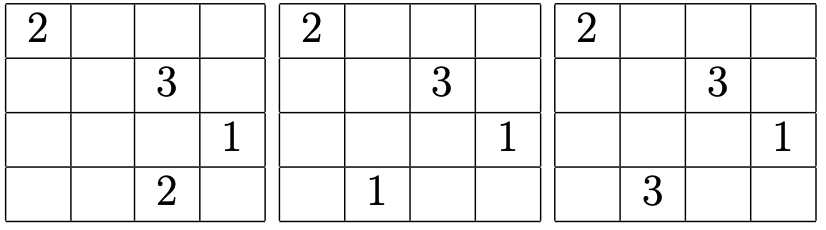
\includegraphics[width=10.0cm]{images/sudoku.png}
    \caption{Рисунок для задачи $5$ и $6$.}
    \label{ris:sudoku}
\end{figure}

\solution{5}
\begin{blockquote}
{\color{myblue}
\noindent C помощью распространения единицы можно решить судоку №$2$. На рисунке~\ref{ris:sudoku_unit} можно видеть, что действительно без каких-либо дополнительных предположений с порождением новых слоев в графе CDCL мы смогли получить решение судоку. Для первого и третьего рисунка так не получится, в них придется вносить дополнительные предположения. (Красным цветом обозначены числа, которые нельзя написать из-за ограничений.) 
\begin{figure}[H]
    \centering
    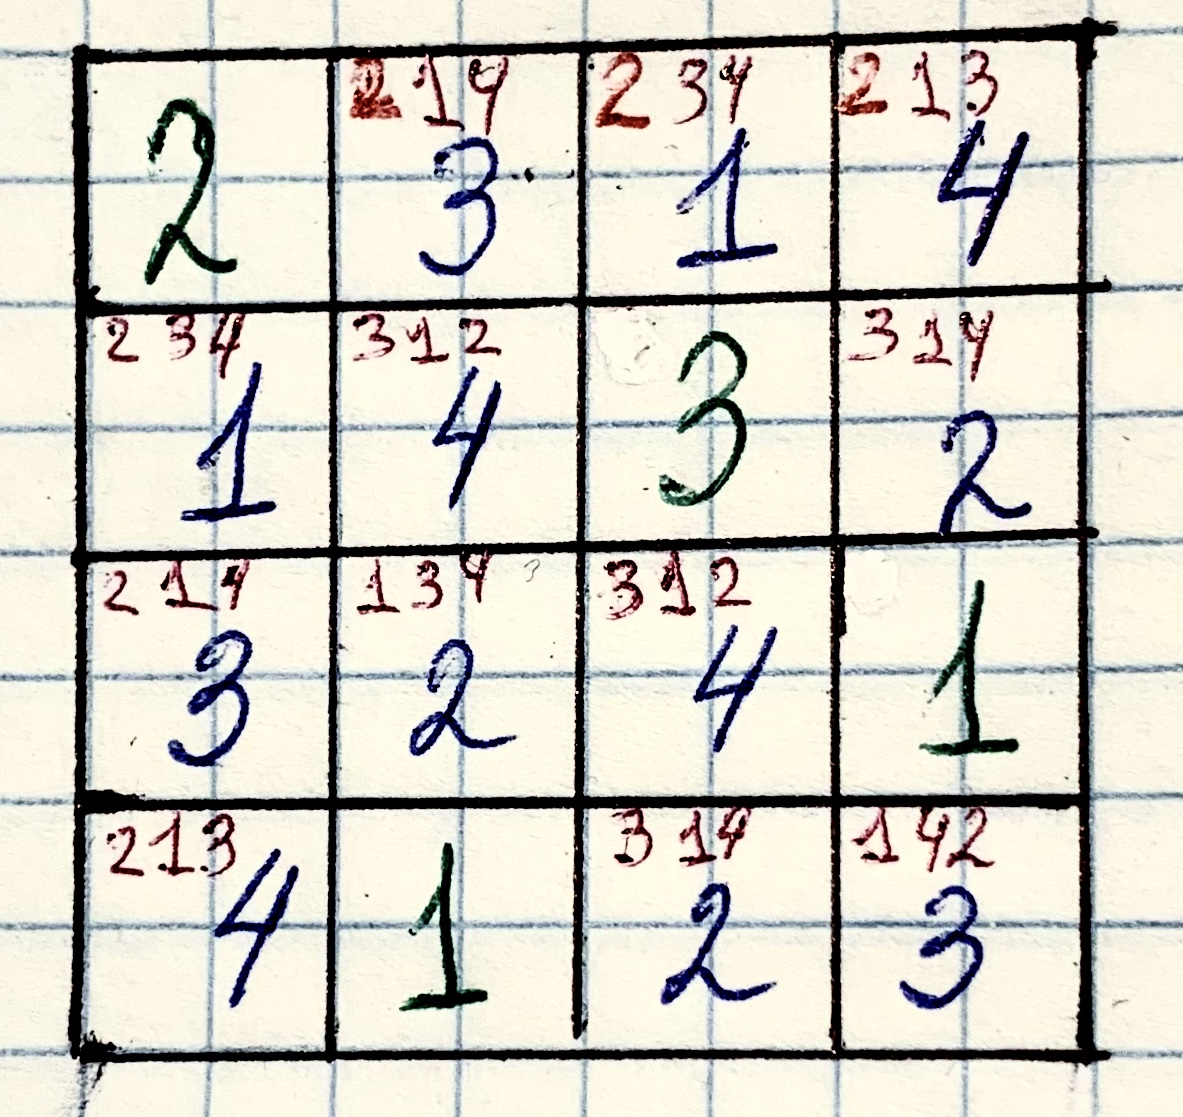
\includegraphics[width=7.0cm]{images/sudoku_unit.JPG}
    \caption{Решение второго судоку с помощью распространения единицы.}
    \label{ris:sudoku_unit}
\end{figure}
}
\end{blockquote}

% Задача №6
\Pr[5 баллов] Рассмотрим три приведенных поля судоку на рисунке~\ref{ris:sudoku}. Какие из них выполнимы? Перечислите все удовлетворяющие оценки полей в виде списка истинных литералов.



\solution{6}
\begin{blockquote}
{\color{myblue}
\noindent Заметим, что можно модифицировать формулу из задачи №$4$, добавив условие на уже присутствующие числа в судоку. Полученную формулу в DIMACS формате уже можно подать на вход солверу.
\begin{figure}[H]
    \centering
    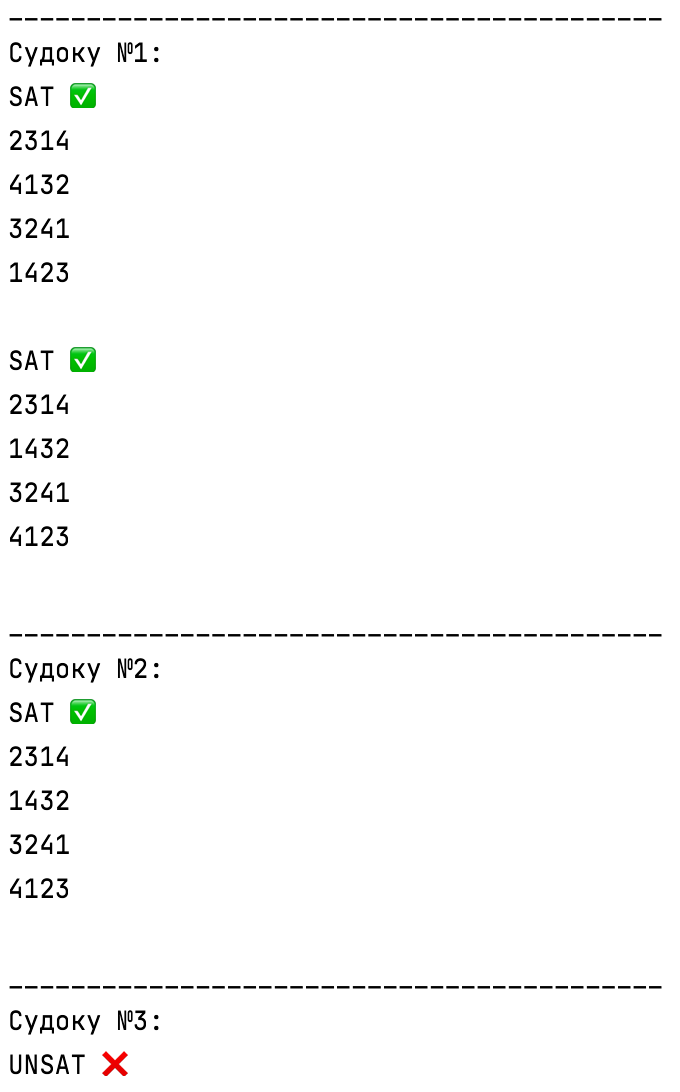
\includegraphics[width=7.0cm]{images/sudoku_solver.png}
    \caption{Вывод программы \textbf{sudoku\_solver.py} в задаче №$6$.}
    \label{ris:sudoku_solver}
\end{figure}
\\
Генератор DIMACS для головоломок $n$-судоку находится в программе\\ {\fcolorbox{red}{myyellow}{06\_sudoku\_solver.py}}.\\
\\
На рисунке~\ref{ris:sudoku_solver} представлен вывод программы для различных судоку с рисунка~\ref{ris:sudoku}.\\
\\
Список истинных литералов очевидно следует из рисунка~\ref{ris:sudoku_solver}. Например, число $1$, находящееся в $3$-ей строке и в $4$-ом столбце первого судоку соответствует истинному литералу $x_{3, 4}^1$.
}
\end{blockquote}
			
			
\end{document}
  